\chapter{ऐमीन और नाइट्रोजन यौगिक}\label{ch:b2:amines}

जो मछली अब ताज़ा नहीं, उससे ट्राइमेथिलऐमीन की गंध आती है, जो एक छोटा वाष्पशील ऐमीन है।
नींबू का थोड़ा रस गंध दूर कर देता है: अम्ल ऐमीन को प्रोटॉनित करता है, और
बना अमोनियम आयन, आयन होने के कारण, वाष्पित नहीं हो सकता। नाइट्रोजन का एकाकी युग्म
ऐमीनों को क्षारक और नाभिकरागी बनाता है; किसी कार्बोनिल से बँधकर वह \omterm{def:b2:amines:imine}{इमीन} देता है,
जिनके माध्यम से प्रोटीन अपना रसायन चलाते हैं और रसायनज्ञ ऐमीन बनाते हैं; और
किसी \omterm{def:b2:huckel:aromatic}{ऐरोमैटिक} वलय पर वह डाइऐज़ोनियम लवणों के माध्यम से उन ऐज़ो रंजकों का मार्ग खोलता है
जिन्होंने उन्नीसवीं शताब्दी को रंगीन किया।

\begin{recall}
प्रथम वर्ष का खंड: ब्रॉन्स्टेड अम्ल और क्षारक, $\mathrm pK_a$ और प्रभाविता आरेख,
नाभिकरागी और द्वि-अणुक प्रतिस्थापन, हेमीऐसीटैल और ऐसीटैल, हाइड्राइड दाता,
कार्बमैग्नीशियम अभिकर्मक, कार्बन की श्रेणी। \Cref{ch:b2:aromatic-substitution}:
नाइट्रीकरण, नाइट्रोऐरीनों का अपचयन। विद्यालय का खंड: ऐमीन और ऐमाइड।
\end{recall}

\begin{omfigure}
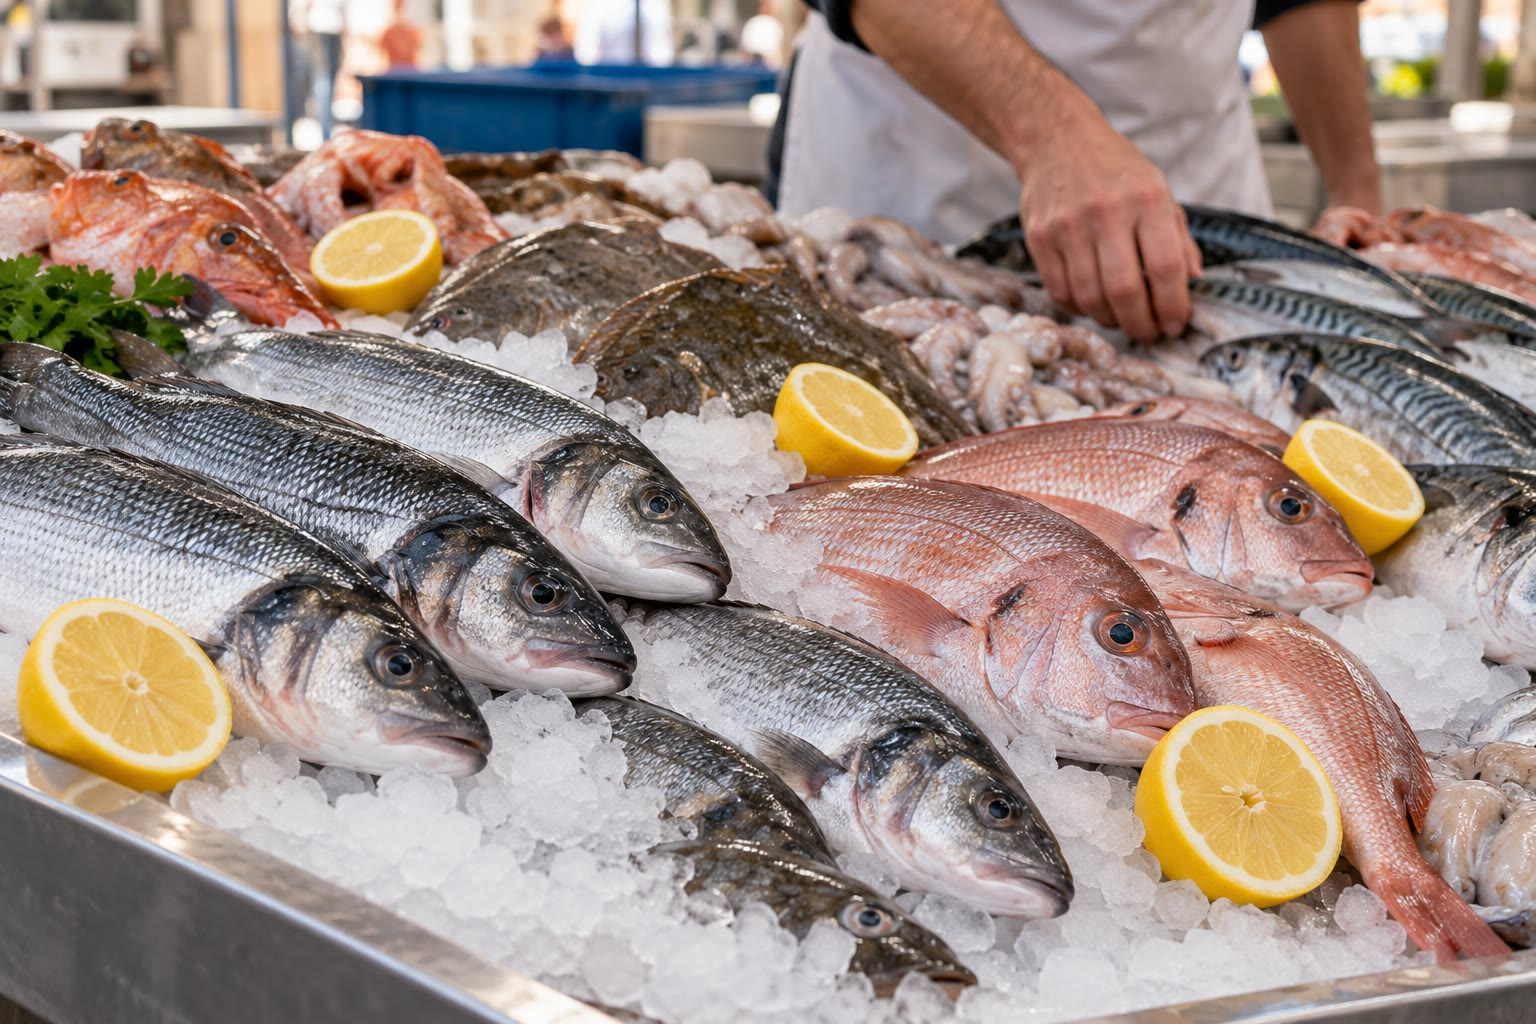
\includegraphics[width=0.6\linewidth]{images/book3/ai/b2-23-fish-stall.jpg}

{\small मछली की एक दुकान: आधे कटे नींबू मछलियों के बीच रखे हैं। उनका अम्ल
मछली के ट्राइमेथिलऐमीन को उसके अवाष्पशील अमोनियम आयन में बदल देता है।}
\end{omfigure}

\section{संरचना और क्षारकता}

\begin{definition}[ऐमीनों की श्रेणियाँ]\label{def:b2:amines:class}
कोई ऐमीन \emph{प्राथमिक ऐमीन}\index{प्राथमिक ऐमीन} \ce{RNH2}, \emph{द्वितीयक ऐमीन}
\index{द्वितीयक ऐमीन} \ce{R2NH} या \emph{तृतीयक ऐमीन}\index{तृतीयक ऐमीन}
\ce{R3N} है, नाइट्रोजन से बँधे कार्बन समूहों की संख्या के अनुसार। \emph{चतुष्क
अमोनियम आयन}\index{चतुष्क अमोनियम आयन} \ce{R4N+} के चार होते हैं, और कोई एकाकी युग्म नहीं।
\end{definition}

ऐमीन का नाइट्रोजन लगभग चतुष्फलकीय होता है, एकाकी युग्म चौथी
स्थिति घेरता है। तीन भिन्न समूहों वाला \omterm{def:b2:amines:class}{तृतीयक ऐमीन} सिद्धांततः किरैल है परंतु उसका
वियोजन नहीं किया जा सकता: अणु एक समतलीय व्यवस्था से होकर प्रतीपित होता है, हवा में छाते की तरह,
कमरे के ताप पर प्रति सेकंड अरबों बार।

\begin{proposition}[क्षारकता]\label{prop:b2:amines:basicity}
जल में ऐल्किलऐमीन अमोनिया से प्रबल क्षारक हैं (उनके अमोनियम आयनों का $\mathrm pK_a$
10 से 11 के निकट, जबकि 9.26), ऐरिलऐमीन कहीं दुर्बल (ऐनिलीनियम 4.60), और ऐमाइड
लगभग बिल्कुल क्षारकीय नहीं (प्रोटॉनित एथेनैमाइड लगभग $-0.6$)।
\end{proposition}

\begin{proof}[तर्क]
ऐल्किल समूह नाइट्रोजन पर इलेक्ट्रॉन घनत्व धकेलते हैं (प्रेरणिक प्रभाव) और
अमोनियम आयन के धनात्मक आवेश को स्थायी करते हैं। जल में हाइड्रोजन आबंधों द्वारा विलायकन भी महत्त्वपूर्ण है:
अधिक \ce{N-H} आबंधों वाले आयन का विलायकन बेहतर होता है, इसीलिए ट्राइमेथिलअमोनियम (9.80)
अमोनियम से दुर्बल अम्ल है परंतु डाइमेथिलअमोनियम (10.73) से प्रबल। ऐनिलीन में एकाकी
युग्म वलय में विस्थानीकृत है और प्रोटॉनन पर खो जाता है; ऐमाइड में वह
कार्बोनिल ऑक्सीजन पर विस्थानीकृत है, और प्रोटॉनन, दुर्बल रूप से, ऑक्सीजन पर होता है।
% ledger: kb:NH3, pka:methylammonium, pka:dimethylammonium, pka:trimethylammonium, pka:anilinium, pka:ethanamideH
\end{proof}

\begin{omfigure}
\begin{tikzpicture}[font=\small, x=0.85cm]
  \draw[->, thick] (-1.5,0) -- (11.8,0) node[below right] {$\mathrm pK_a$};
  \foreach \x in {0,2,4,6,8,10} \draw (\x,0.1) -- (\x,-0.1) node[below, font=\scriptsize] {\x};
  \foreach \x/\l in {-0.6/{\ce{CH3CONH3+}}, 4.60/{\ce{C6H5NH3+}}} {
    \draw[omDef, thick] (\x,0) -- (\x,0.5);
    \node[font=\scriptsize, anchor=south] at (\x,0.5) {\l};
  }
  \foreach \x/\l/\y/\h in {9.26/{\ce{NH4+} (9.26)}/1.95/1.2, 9.80/{\ce{(CH3)3NH+} (9.80)}/1.45/0.85, 10.66/{\ce{CH3NH3+} (10.66)}/0.95/0.5, 10.73/{\ce{(CH3)2NH2+} (10.73)}/0.45/0.25} {
    \draw[omDef, thick] (\x,0) -- (\x,\h);
    \draw[black!40] (\x,\h) -- (12.2,\y);
    \node[font=\scriptsize, anchor=west] at (12.2,\y) {\l};
  }
  \node[font=\scriptsize, anchor=north west] at (-1.4,-0.5) {दुर्बलतर क्षारक};
  \node[font=\scriptsize, anchor=north east] at (11.7,-0.5) {प्रबलतर क्षारक};
\end{tikzpicture}

{\small कुछ नाइट्रोजन क्षारकों के संयुग्मी अम्लों का \qty{25}{\degreeCelsius} पर
$\mathrm pK_a$: यह जितना ऊँचा, क्षारक उतना प्रबल।}
% ledger: kb:NH3, pka:methylammonium, pka:dimethylammonium, pka:trimethylammonium, pka:anilinium, pka:ethanamideH
\end{omfigure}

\section{नाभिकरागी के रूप में ऐमीन}

ऐमीन द्वि-अणुक प्रतिस्थापन द्वारा हैलोऐल्केनों पर आक्रमण करते हैं। उत्पाद, एक अधिक प्रतिस्थापित
ऐमीन, कम-से-कम आरंभिक ऐमीन जितना नाभिकरागी होता है और हैलोऐल्केन के लिए प्रतिस्पर्धा करता है:
अमोनिया का ऐल्किलन प्राथमिक, द्वितीयक और \omterm{def:b2:amines:class}{तृतीयक ऐमीनों} तथा
चतुष्क लवण का मिश्रण देता है।

\begin{proposition}[बहु-ऐल्किलन]\label{prop:b2:amines:polyalkylation}
अमोनिया या किसी \omterm{def:b2:amines:class}{प्राथमिक ऐमीन} का प्रत्यक्ष ऐल्किलन मिश्रण देता है; केवल चतुष्क
अमोनियम लवण तक का पूर्ण ऐल्किलन स्वच्छ होता है।
\end{proposition}

\begin{proof}[तर्क]
हर ऐल्किलन ऐसे नाइट्रोजन पर एक एकाकी युग्म छोड़ता है जो नए ऐल्किल समूह से अधिक
इलेक्ट्रॉन-समृद्ध हो गया है; उत्पाद शेष हैलोऐल्केन से तुलनीय दर पर अभिक्रिया करता है। केवल जब
नाइट्रोजन पर कोई एकाकी युग्म नहीं बचता, \ce{R4N+} में, तभी अनुक्रम रुकता है।
\end{proof}

अति-ऐल्किलित संबंधियों से मुक्त \omterm{def:b2:amines:class}{प्राथमिक ऐमीन} अप्रत्यक्ष रूप से बनाए जाते हैं: गेब्रियल
मार्ग से (थैलिमाइड के नाइट्रोजन का ऐल्किलन, जिस पर एक ही अम्लीय हाइड्रोजन होता है, फिर
ऐमीन की मुक्ति), किसी \omterm{def:b2:amines:nitrile}{नाइट्राइल}, किसी ऐमाइड या किसी नाइट्रो यौगिक के अपचयन से, या
\omterm{def:b2:amines:reductive-amination}{अपचायी ऐमीनन} से (नीचे)।

\section{इमीन और एनामीन}

\begin{definition}[नाभिकरागी योग]\label{def:b2:amines:nucleophilic-addition}
किसी कार्बोनिल समूह पर \emph{नाभिकरागी योग}\index{नाभिकरागी योग} कार्बोनिल कार्बन पर
किसी नाभिकरागी का आक्रमण है, जिससे वह कार्बन चतुष्फलकीय हो जाता है और \ce{C=O} $\pi$ आबंध
ऑक्सीजन पर एक एकाकी युग्म बन जाता है।
\end{definition}

\begin{definition}[हेमीऐमिनल, इमीन और एनामीन]\label{def:b2:amines:imine}
कोई \omterm{def:b2:amines:class}{प्राथमिक ऐमीन} किसी ऐल्डिहाइड या कीटोन से जुड़कर \emph{हेमीऐमिनल}\index{हेमीऐमिनल}
देता है (\ce{OH} और \ce{NHR} धारण करने वाला कार्बन); इसका निर्जलीकरण \emph{इमीन}\index{इमीन}
$\mathrm{R_2C{=}NR'}$ देता है। कोई \omterm{def:b2:amines:class}{द्वितीयक ऐमीन}, जो उदासीन इमीन नहीं बना सकता, निर्जलीकरण के बाद
\emph{एनामीन}\index{एनामीन} $\mathrm{R_2C{=}CR{-}NR'_2}$ देता है, द्वि-आबंध सन्निकट कार्बन पर खिसक जाता है।
\end{definition}

\begin{omfigure}
\setchemfig{atom sep=1.9em}
\schemestart
\chemfig{R_2C=O} \+ \chemfig{H_2N-R'}
\arrow{<=>}
\chemfig{R_2C(-[2]OH)-NH-R'}
\arrow{<=>[\ce{H+}][$-$ \ce{H2O}]}
\chemfig{R_2C=N-R'}
\schemestop
\par\vspace{6pt}

{\small \omterm{def:b2:amines:imine}{इमीन} का बनना: कार्बोनिल पर ऐमीन का \omterm{def:b2:amines:nucleophilic-addition}{नाभिकरागी योग}
\omterm{def:b2:amines:imine}{हेमीऐमिनल} देता है; अम्ल उत्प्रेरण उसके \ce{OH} को निर्गामी समूह (\ce{-OH2+}) में बदलता है, जल निकलता है और
नाइट्रोजन का एकाकी युग्म \ce{C=N} द्वि-आबंध बनाता है। हर चरण उत्क्रमणीय है: आधिक्य जल
\omterm{def:b2:amines:imine}{इमीन} का वापस जल-अपघटन कर देता है।}
\end{omfigure}

\begin{proposition}[इष्टतम pH]\label{prop:b2:amines:imine-ph}
\omterm{def:b2:amines:imine}{इमीन} सबसे तेज़ी से मंद अम्लीय विलयन में, pH 4 से 5 के निकट, बनते हैं।
\end{proposition}

\begin{proof}[तर्क]
पहले चरण को मुक्त ऐमीन (उसका एकाकी युग्म) चाहिए; अधिक अम्लीय माध्यम ऐमीन को
प्रोटॉनित कर देता है ($\mathrm pK_a$ लगभग 10) और नाभिकरागी को हटा देता है। निर्जलीकरण को
हाइड्रॉक्सिल समूह को प्रोटॉनित करने के लिए अम्ल चाहिए; उच्च pH पर यह धीमा है। दर, दोनों आवश्यकताओं का गुणनफल,
बीच में सबसे बड़ी होती है।
\end{proof}

\begin{definition}[अपचायी ऐमीनन]\label{def:b2:amines:reductive-amination}
\emph{अपचायी ऐमीनन}\index{अपचायी ऐमीनन} किसी कार्बोनिल यौगिक और किसी
ऐमीन को अधिक प्रतिस्थापित ऐमीन में बदलता है, \omterm{def:b2:amines:imine}{इमीन} (या इमीनियम आयन) बनाकर और उसी पात्र में
उसका अपचयन करके, प्रायः सोडियम सायनोबोरोहाइड्राइड \ce{NaBH3CN} से।
\end{definition}

\begin{proposition}[अपचायी ऐमीनन की वरणात्मकता]\label{prop:b2:amines:reductive-amination}
pH 6 के निकट \ce{NaBH3CN} इमीनियम आयन का अपचयन कार्बोनिल यौगिक से कहीं तेज़ी से करता है, जिससे
ऐल्डिहाइड या कीटोन का ऐल्कोहॉल में अपचयन किए बिना ऐमीन बन जाता है।
\end{proposition}

\begin{proof}[तर्क]
सायनो समूह \ce{BH3CN-} को दुर्बल हाइड्राइड दाता बनाता है, जो उदासीन कार्बोनिल के लिए बहुत दुर्बल है परंतु
प्रोटॉनित, धनावेशित इमीनियम आयन के लिए पर्याप्त, जो कहीं बेहतर इलेक्ट्रॉनरागी है।
\end{proof}

\section{डाइऐज़ोनियम लवण}

\begin{definition}[डाइऐज़ोनियम रसायन]\label{def:b2:amines:diazonium}
\emph{डाइऐज़ोनियम आयन}\index{डाइऐज़ोनियम आयन} एक धनायन \ce{R-N+#N} है। \emph{डाइऐज़ोकरण}\index{डाइऐज़ोकरण}
किसी प्राथमिक \omterm{def:b2:huckel:aromatic}{ऐरोमैटिक} ऐमीन को सोडियम नाइट्राइट और किसी प्रबल अम्ल से
0--\qty{5}{\degreeCelsius} पर ऐरिल डाइऐज़ोनियम लवण में बदलता है। \emph{सांडमेयर अभिक्रिया}\index{सांडमेयर अभिक्रिया} में कोई कॉपर(I) लवण
(\ce{CuCl}, \ce{CuBr}, \ce{CuCN}) डाइनाइट्रोजन की हानि के साथ डाइऐज़ोनियम समूह को Cl, Br या CN से
प्रतिस्थापित करता है। \emph{ऐज़ो युग्मन}\index{ऐज़ो युग्मन} में डाइऐज़ोनियम आयन, एक दुर्बल इलेक्ट्रॉनरागी,
किसी सक्रियित \omterm{def:b2:huckel:aromatic}{ऐरोमैटिक} वलय पर आक्रमण करके ऐज़ो यौगिक $\mathrm{Ar{-}N{=}N{-}Ar'}$ देता है।
\end{definition}

\begin{proposition}[डाइऐज़ोनियम आयनों का स्थायित्व]\label{prop:b2:amines:diazonium}
ऐरिल डाइऐज़ोनियम लवण ठंडे जलीय विलयन में रखे और प्रयुक्त किए जा सकते हैं; ऐल्किल \omterm{def:b2:amines:diazonium}{डाइऐज़ोनियम आयन}
तुरंत डाइनाइट्रोजन खो देते हैं।
\end{proposition}

\begin{proof}[तर्क]
डाइनाइट्रोजन एक उत्कृष्ट निर्गामी समूह है (अत्यंत स्थायी अणु, एन्ट्रॉपी में बड़ा लाभ)।
ऐल्किल समूह के लिए \ce{N2} की हानि एक कार्बधनायन छोड़ती है, या जल सीधे आक्रमण करता है: आयन
टिकता नहीं। ऐरिल धनायन अत्यंत अस्थायी है (वलय के तल में एक खाली $\sigma$ कक्षक,
जो $\pi$ निकाय से स्थायीकृत नहीं), और ऐरिल \omterm{def:b2:amines:diazonium}{डाइऐज़ोनियम आयन} का \ce{C-N} आबंध
वलय के साथ संयुग्मन से प्रबल होता है: निम्न ताप पर वह बना रहता है; गर्म करने पर वह विघटित होता है,
और जल डाइऐज़ोनियम समूह को \ce{OH} से प्रतिस्थापित कर देता है।
\end{proof}

\begin{omfigure}
\begin{tikzpicture}[font=\small, >={Stealth}]
  \node[cyclenode] (d) at (0,0) {\ce{Ar-N2+}};
  \foreach \a/\t/\c in {90/{\ce{Ar-Cl}}/{\ce{CuCl}}, 150/{\ce{Ar-Br}}/{\ce{CuBr}}, 210/{\ce{Ar-CN}}/{\ce{CuCN}},
                        270/{\ce{Ar-OH}}/{\ce{H2O}, गर्म}, 330/{\ce{Ar-H}}/{\ce{H3PO2}}, 30/{$\mathrm{Ar{-}N{=}N{-}Ar'}$}/{सक्रियित \ce{ArH}}} {
    \node[cyclenode] (p\a) at (\a:2.6) {\t};
    \draw[->, thick] (d) -- (p\a) node[midway, font=\scriptsize, fill=white, inner sep=1pt] {\c};
  }
\end{tikzpicture}

{\small किसी ऐरिल डाइऐज़ोनियम लवण की अभिक्रियाएँ। \ce{N2+} समूह हैलोजन या
सायनाइड (सांडमेयर, कॉपर(I) लवण) से, \ce{OH} (गर्म जल) से या H (हाइपोफ़ॉस्फ़ोरस अम्ल) से प्रतिस्थापित होता है, या
\omterm{def:b2:amines:diazonium}{ऐज़ो युग्मन} में बना रहता है।}
\end{omfigure}

\begin{method}[डाइऐज़ोनियम लवण से होकर जाने वाले मार्ग]\label{met:b2:amines:diazonium-routes}
\begin{enumerate}
  \item अन्य समूहों को रखने के लिए ऐमीनो समूह (एक प्रबल \omterm{def:b2:aromatic-substitution:directing}{ऑर्थो/पैरा निर्देशक}) का उपयोग कीजिए, फिर उसे
        डाइऐज़ोनियम लवण के माध्यम से बदल दीजिए।
  \item उसे H से प्रतिस्थापित करके ऐसे पैटर्न पाइए जो प्रत्यक्ष प्रतिस्थापन नहीं दे सकता
        (ऐनिलीन से 1,3,5-ट्राइब्रोमोबेन्ज़ीन)।
  \item उसे CN से प्रतिस्थापित कीजिए, फिर जल-अपघटन से कार्बोक्सिलिक अम्ल बनाइए: वलय पर \ce{-COOH} पाने का एक तरीका।
\end{enumerate}
\end{method}

\begin{method}[ऐमीन बनाना]\label{met:b2:amines:make-amine}
\begin{enumerate}
  \item ऐल्किल शृंखला पर \omterm{def:b2:amines:class}{प्राथमिक ऐमीन}: गेब्रियल मार्ग, या किसी \omterm{def:b2:amines:nitrile}{नाइट्राइल} का अपचयन (उसे बनाने में प्रयुक्त
        हैलोऐल्केन से एक कार्बन अधिक) या किसी ऐमाइड का।
  \item द्वितीयक या \omterm{def:b2:amines:class}{तृतीयक ऐमीन}: सही कार्बोनिल यौगिक का सही ऐमीन के साथ
        \omterm{def:b2:amines:reductive-amination}{अपचायी ऐमीनन}।
  \item \omterm{def:b2:huckel:aromatic}{ऐरोमैटिक} ऐमीन: नाइट्रीकरण, फिर अपचयन (अम्ल के साथ आयरन या टिन, या \omterm{def:b2:alkene-redox:hydrogenation}{उत्प्रेरकी
        हाइड्रोजनन})।
\end{enumerate}
\end{method}

\section{नाइट्राइल}

\begin{definition}[नाइट्राइल]\label{def:b2:amines:nitrile}
\emph{नाइट्राइल}\index{नाइट्राइल} एक यौगिक \ce{R-C#N} है, जो सायनाइड द्वारा किसी हैलोऐल्केन के प्रतिस्थापन से
या \omterm{def:b2:amines:diazonium}{सांडमेयर अभिक्रिया} से बनता है।
\end{definition}

\begin{proposition}[नाइट्राइलों की अभिक्रियाएँ]\label{prop:b2:amines:nitrile}
\omterm{def:b2:amines:nitrile}{नाइट्राइल} का, अम्ल या क्षारक में, ऐमाइड तक और फिर कार्बोक्सिलिक अम्ल तक जल-अपघटन होता है; लिथियम
ऐलुमिनियम हाइड्राइड उसे \omterm{def:b2:amines:class}{प्राथमिक ऐमीन} \ce{RCH2NH2} में अपचित करता है; कोई कार्बमैग्नीशियम
अभिकर्मक उससे एक बार जुड़ता है, और बने \omterm{def:b2:amines:imine}{इमीन} का जल-अपघटन एक कीटोन देता है।
\end{proposition}

\begin{proof}[तर्क]
\omterm{def:b2:amines:nitrile}{नाइट्राइल} कार्बन, कार्बोनिल कार्बन की तरह, इलेक्ट्रॉनरागी है: जल (अम्ल से सक्रियित, या
हाइड्रॉक्साइड के रूप में) उससे जुड़ता है, और चलावयवता के बाद एक ऐमाइड देता है, जिसके जल-अपघटन का विवेचन
\cref{ch:b2:acyl-substitution} में है। हाइड्राइड दो बार जुड़ता है। कार्बमैग्नीशियम अभिकर्मक एक बार जुड़ता है,
और एक \omterm{def:b2:amines:imine}{इमीन} ऋणायन देता है जो आगे अभिक्रिया नहीं करता; फिर जल \omterm{def:b2:amines:imine}{इमीन} का जल-अपघटन करके कीटोन देता है।
\end{proof}

\begin{safety}{\ghs[5mm]{GHS03}\,\ghs[5mm]{GHS06}\,\ghs[5mm]{GHS08}\,\ghs[5mm]{GHS09}}
ऐनिलीन और \textit{N},\textit{N}-डाइमेथिलऐनिलीन त्वचा-संपर्क से विषैले हैं; सोडियम नाइट्राइट
विषैला और ऑक्सीकारक है; सोडियम सायनोबोरोहाइड्राइड अम्ल में हाइड्रोजन सायनाइड मुक्त करता है और उसे
धूम-हुड में प्रयुक्त करना चाहिए। शुष्क डाइऐज़ोनियम लवण विस्फोट कर सकते हैं: उन्हें सदैव ठंडे, विलयन में रखा जाता है, और
तुरंत प्रयुक्त किया जाता है।
% ledger: ghs:aniline, ghs:dimethylaniline, ghs:NaNO2, ghs:NaBH3CN, ghs:sulfanilic-acid
\end{safety}

\section{अभ्यास}

\begin{exercise}[$\star$]\label{exo:b2:amines:1}
श्रेणी बताइए: प्रोपेन-1-ऐमीन, \textit{N}-मेथिलएथेनैमीन, ट्राइएथिलऐमीन,
टेट्रामेथिलअमोनियम क्लोराइड, ऐनिलीन।
\end{exercise}

\begin{exercise}[$\star$]\label{exo:b2:amines:2}
बढ़ती क्षारकता के क्रम में रखिए: अमोनिया, मेथिलऐमीन, ऐनिलीन, एथेनैमाइड।
\end{exercise}

\begin{exercise}[$\star$]\label{exo:b2:amines:3}
साइक्लोहेक्सेनोन और मेथिलऐमीन से बनने वाला \omterm{def:b2:amines:imine}{इमीन}, और परिस्थितियाँ, दीजिए।
\end{exercise}

\begin{exercise}[$\star$]\label{exo:b2:amines:4}
बेन्ज़ीनडाइऐज़ोनियम क्लोराइड से आरंभ करके \ce{CuBr}, \ce{CuCN}, गर्म जल,
और क्षारक में फ़ीनॉल के साथ उत्पाद दीजिए।
\end{exercise}

\begin{exercise}[$\star\star$]\label{exo:b2:amines:5}
pH 7 पर ट्राइमेथिलऐमीन का कौन-सा रूप प्रभावी है, और किस अनुपात में? नींबू की व्याख्या कीजिए, और यह भी कि किसी
ऐमीन को कार्बनिक विलायक से जल में कैसे निष्कर्षित किया जा सकता है।
\end{exercise}

\begin{exercise}[$\star\star$]\label{exo:b2:amines:6}
साइक्लोहेक्सेनोन और पिरोलिडीन से बनने वाला \omterm{def:b2:amines:imine}{एनामीन} दीजिए, और समझाइए कि \omterm{def:b2:amines:class}{द्वितीयक ऐमीन}
\omterm{def:b2:amines:imine}{इमीन} क्यों नहीं दे सकता।
\end{exercise}

\begin{exercise}[$\star\star$]\label{exo:b2:amines:7}
\omterm{def:b2:amines:reductive-amination}{अपचायी ऐमीनन} द्वारा \textit{N}-बेन्ज़िलप्रोपेन-2-ऐमीन \ce{C6H5CH2NHCH(CH3)2} बनाइए: अभिकर्मकों के दो
संभावित युग्म दीजिए।
\end{exercise}

\begin{exercise}[$\star\star$]\label{exo:b2:amines:8}
बेन्ज़ोनाइट्राइल एथिलमैग्नीशियम ब्रोमाइड से, फिर जलीय अम्ल से अभिक्रिया करता है। उत्पाद दीजिए।
\end{exercise}

\begin{exercise}[$\star\star$]\label{exo:b2:amines:9}
हेक्सेन-1-ऐमीन का गेब्रियल संश्लेषण लिखिए और समझाइए कि यह कोई \omterm{def:b2:amines:class}{द्वितीयक ऐमीन} क्यों नहीं देता।
\end{exercise}

\begin{exercise}[$\star\star\star$]\label{exo:b2:amines:10}
ऐनिलीन से 1,3,5-ट्राइब्रोमोबेन्ज़ीन बनाइए।
\end{exercise}

\begin{exercise}[$\star\star\star$]\label{exo:b2:amines:11}
4-नाइट्रोऐनिलीन और फ़ीनॉल से एक ऐज़ो रंजक की रूपरेखा बनाइए: \omterm{def:b2:amines:diazonium}{डाइऐज़ोकरण}, युग्मन (स्थिति
और pH), और उत्पाद लिखिए।
\end{exercise}

\begin{exercise}[$\star\star\star$]\label{exo:b2:amines:12}
\textit{N},\textit{N}-डाइमेथिलब्यूटेन-2-ऐमीन का चतुष्क अमोनियम हाइड्रॉक्साइड गर्म करने पर
अधिकांशतः ब्यूट-1-ईन देता है। इस हॉफ़मान अभिविन्यास को समझाइए, जो प्रथम वर्ष के
खंड के ज़ैत्सेव के नियम के विपरीत है।
\end{exercise}

\section{समस्या: मेथिल ऑरेंज बनाना}

\begin{problem}[{सप्ताहांत समस्या --- सल्फ़ैनिलिक अम्ल और उसका \omterm{def:b2:amines:diazonium}{डाइऐज़ोकरण},
\textit{N},\textit{N}-डाइमेथिलऐनिलीन के साथ \omterm{def:b2:amines:diazonium}{ऐज़ो युग्मन}, सूचक के रूप में मेथिल ऑरेंज, और लब्धि}]
\label{pb:b2:amines:1}
आँकड़े: सल्फ़ैनिलिक अम्ल (4-ऐमीनोबेन्ज़ीनसल्फ़ोनिक अम्ल) \ce{C6H7NO3S}; मेथिल ऑरेंज, सोडियम लवण
\ce{C14H14N3NaO3S}; मेथिल ऑरेंज के अम्ल रूप का $\mathrm pK_a$ 3.47। मोलर द्रव्यमान
(\unit{g/mol}): C 12.011, H 1.008, N 14.007, O 15.999, Na 22.990, S 32.06। प्रयोग (अभ्यास के आँकड़े):
सल्फ़ैनिलिक अम्ल के \qty{5.00}{g}, लब्धि 80~\%।
% ledger: pka:methylorange, aw:C, aw:H, aw:N, aw:O, aw:Na, aw:S, ghs:sulfanilic-acid, ghs:NaNO2

\medskip
\noindent\textbf{भाग I --- सल्फ़ैनिलिक अम्ल और \omterm{def:b2:amines:diazonium}{डाइऐज़ोकरण}।}
\begin{enumerate}
  \item सल्फ़ैनिलिक अम्ल उभयाविष्ट आयन के रूप में रहता है। उसे खींचिए।
  \item इसे पहले सोडियम कार्बोनेट विलयन में क्यों घोला जाता है?
  \item सोडियम नाइट्राइट और हाइड्रोक्लोरिक अम्ल से नाइट्रस अम्ल का बनना लिखिए।
  \item 4-सल्फ़ोनेटोऐनिलीनियम आयन का \omterm{def:b2:amines:diazonium}{डाइऐज़ोकरण} लिखिए।
  \item अभिक्रिया 0--\qty{5}{\degreeCelsius} पर क्यों चलाई जाती है?
  \item सल्फ़ैनिलिक अम्ल के \qty{5.00}{g} के लिए सोडियम नाइट्राइट की कितनी मात्रा चाहिए?
  \item नाइट्राइट के हल्के आधिक्य का परीक्षण क्यों किया जाता है, और उसे नष्ट क्यों किया जाता है?
\end{enumerate}

\medskip
\noindent\textbf{भाग II --- युग्मन।}
\begin{enumerate}[resume]
  \item \textit{N},\textit{N}-डाइमेथिलऐनिलीन एक अच्छा भागीदार क्यों है?
  \item \omterm{def:b2:amines:diazonium}{डाइऐज़ोनियम आयन} उसके वलय की किस स्थिति पर आक्रमण करता है, और क्यों?
  \item उत्पाद लिखिए (सल्फ़ोनेट के रूप में)।
  \item युग्मन दुर्बल अम्लीय, न कि प्रबल अम्लीय, विलयन में क्यों चलाया जाता है?
  \item सोडियम लवण को अवक्षेपित करने के लिए फिर विलयन को क्षारीय क्यों बनाना पड़ता है?
  \item \omterm{def:b2:amines:diazonium}{डाइऐज़ोनियम आयन} दुर्बल इलेक्ट्रॉनरागी क्यों है, जो केवल सक्रियित वलयों से अभिक्रिया करता है?
\end{enumerate}

\medskip
\noindent\textbf{भाग III --- एक सूचक।}
\begin{enumerate}[resume]
  \item क्षारक में और अम्ल में मेथिल ऑरेंज किस रंग का होता है?
  \item यह प्रोटॉन कहाँ ग्रहण करता है?
  \item इसका रंग किस pH परास में बदलता है?
  \item विस्तारित संयुग्मित निकाय दृश्य रंग क्यों देता है?
  \item प्रोटॉनन अवशोषण को क्यों खिसका देता है?
\end{enumerate}

\medskip
\noindent\textbf{भाग IV --- लब्धि।}
\begin{enumerate}[resume]
  \item सल्फ़ैनिलिक अम्ल का मोलर द्रव्यमान परिकलित कीजिए।
  \item मेथिल ऑरेंज (सोडियम लवण) का मोलर द्रव्यमान परिकलित कीजिए।
  \item प्रयुक्त सल्फ़ैनिलिक अम्ल की मात्रा परिकलित कीजिए।
  \item मेथिल ऑरेंज का सैद्धांतिक द्रव्यमान परिकलित कीजिए।
  \item कौन-सी हानियाँ 100~\% से कम लब्धि की व्याख्या करती हैं?
  \item 80~\% लब्धि पर सल्फ़ैनिलिक अम्ल के \qty{5.00}{g} से प्राप्त मेथिल ऑरेंज का द्रव्यमान
        बताइए।
\end{enumerate}
\end{problem}
